\chapter{Pharmacokinetic modelling}
\label{chapter:pk}

The ideal output obtained from DCE-MRI analysis would be some reliable quantitative physiological parameters of the tissue under examination. Numerical results, however, always call for some mathematical description of the system under examination. 

The time-dependent distribution and deposition of a substance in a living system can be described by Phamacokinetic (PK) models~\cite{gerlowski1983physiologically}. First attempts of depicting the organism by a set of components were performed by Torsten Teorell in 1937. He then created a model of whole body shown in Figure \ref{fig:pk_draft} and decried the processes inside by a set of diferentail equations in the same time presenting  their solutions~\cite{pkfather}. Teorell is now considered  a father of \textit{Pharmacokinetic} (PK) modelling. 

\begin{figure}[t]
		\centering
		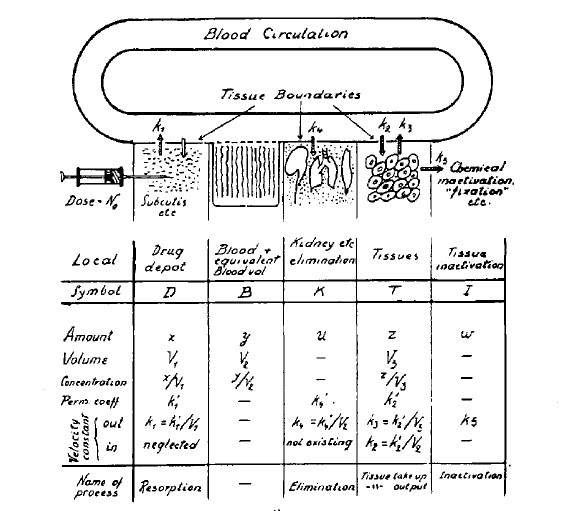
\includegraphics[height =11cm]{pk_draft}
		\caption [Teorell first PK model]{First PK model desribed by Teorell \cite{pk_draft}}
		\label{fig:pk_draft}
	\end{figure}

PK models aim to characterise a physiologic system, not nesseserly the whole body, by decomposing it into interacting compartments. Every of them is a homogenous, well-mixed space with the uniform tracer distribution \cite{PMID:20540902}.
Thus, the multicompartment system reaches the equilibrum in different time.  PK models have very wide clinical application: from estimating the optimal drug dose to determining safe working environment while working with toxins  \cite{gerlowski1983physiologically}.

Given the fact that the contrast agent used in DCE-MRI examination can be considered as a substance flowing through the organism, Pharmacokintetic modelling can also be used in analysis of so obtained data.   
This approach, called the quantitative one, is based on fitting mathematical model to acquired tissue concentration time courses. In this way, the quantitative parameters can be assessed, which cannot be overestimated while evaluating the tissue function. 


This chapter deals with the approach of PK modelling giving the brief inside in its basic principles and requirements with focus on DCE-MRI applications. 
\newpage



\section{The tracer kinetic theory} 
The compartment PK models describe complex blood-tissue exchanges. The general tracer kinetic theory is based on mass conservation principle and PK models are formulated as mass balance equations. 
\begin{figure}[H]
\captionsetup[subfloat]{captionskip=0.5cm}
	\centering
	\subfloat [An arbitrary tissue]{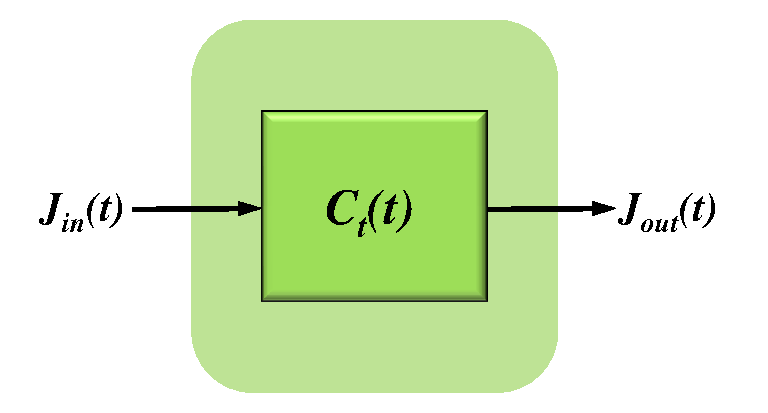
\includegraphics[width=0.5\linewidth]{model1}\label{fig:model1}}
	\subfloat[An arbitrary two compartment model]{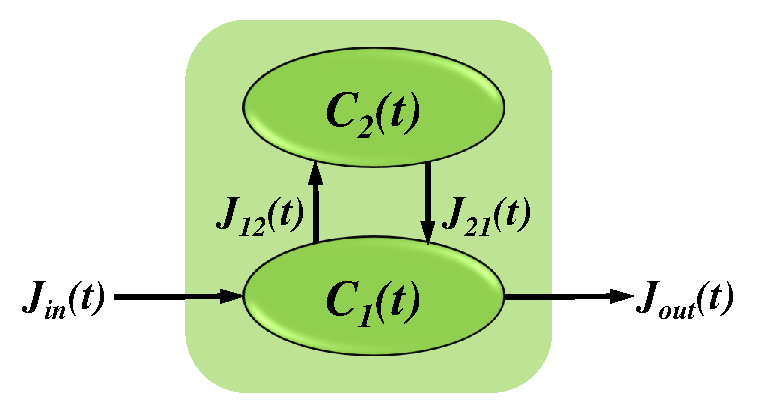
\includegraphics[width=0.5\linewidth]{model2}\label{fig:model2}}\\	
\vspace{0.5cm}
\caption[ddd]{aa}
\label{fig:model}
\end{figure}
\noindent Given the tissue with with at least one inlet and one outlet, see Figure~\ref{fig:model}a, the time-varying tracer concentration in the tissue, $C_t(t)$ can be expressed as:
\begin{equation}
C_t(t) = \frac{M_t(t)}{V_t},
\label{eq:pk1}
\end{equation}
where $M_t(t)$ is the amount of tracer in the tissue (in mmol) and $V_t$ is the volume of the tissue (mL). The \textit{flux} (mmol/mL/min) in terms, is the amount of the tracer, which travels through an inlet or outlet per unit time. After the normalisation to the unit tissue volume the flux can be expressed as:
\begin{equation}
J(t) = \frac{1}{V_t}\frac{\partial M_t(t)}{\partial t}
\label{eq:pk2}
\end{equation} 
Let' now consider an arbitrary multi-compartment model composed of $n$ interacting compartments. Then, the outlet of one compartment is in the same time the inlet of another, see Figure~\ref{fig:model}b. The tissue concentration in such a system is defined by:   
\begin{equation}
C_t(t) = \sum_{j=1}^{n}v_jC_j(t),
\label{eq:pk3}
\end{equation}
where $v_j\leq1$ is the \textit{fractional volume} (dimensionless) of $j$th compartment and $C_j$ is the concentration of tracer in this compartment. 
From the principle of the conservation of the mass it is known that no amount of the indicator is neither created nor destroyed in the tissue. Under such condition, applying the mass balance equation to the every of the compartments, the change of the total amount of substance in the compartment is given by:
\begin{equation}
\frac{dM_j(t)}{dt} = \sum_{i}^{I}\frac{M_i(t)}{\partial t}-\sum_{o}^{O}\frac{M_o(t)}{\partial t} ,
\label{eq:pk4}
\end{equation}
where $I$ and $O$ are the number of inlets and outlets of the compartment respectively. 
After normalisation to the unit tissue volume:
\begin{equation}
vj\frac{dC_j(t)}{dt} = \sum_{i}^{I}J_i(t)-\sum_{o}^{O}J_o(t) ,
\label{eq:pk5}
\end{equation}
The mass conservation principle implies that the amount of the substance transported from a compartment $i$ to a compartment $j$ per unit time is equal to the amount of the given substance leaving the $i$. This leads to the formula:
\begin{equation}
\frac{\partial M_{ij}(t)}{\partial t} = k_{ep}M_i,
\label{eq:pk6}
\end{equation}
where $k_{ep}$ is so called \textit{rate constant} (in min$^{-1}$). Again, after the normalisation to the unit tissue volume:
\begin{equation}
J_{ij}(t) = K_{trans}C_i(t),
\label{eq:pk7}
\end{equation}
where $K_{trans}=k_{ep}v_j$ is \textit{transfer constant} (in ml$^{-1}$). $K_{trans}$ combines both the flow and tissue permeability. Some models allow their separate estimation by differentiating the \textit{flow} $F$ by the \textit{permeability surface area product}, $PS$. 

\subsection{Linear stationary systems}
All PK models are based on two fundamental assumptions, without which solving the models' equations would not be possible: that the system is linear and stationary. Hence the response of the influx is proportional to the dose of the injected tracer.  

For any linear and stationary system satisfying the 
initial condition $C_t(0) = 0$, which means $t = 0$ is chosen before tracer injection,
the tissue concentration can be obtained by convolving the concentration of tracer input function with the Impulse Response Function (IRF) of the tissue denotated as $h(t)$ \cite{sourbron2011scope}: 
\begin{equation}
	\label{eq:convolution}
	C_{t}(t) = C_{in}(t)\circledast h(t) = \int_{0}^{t}C_{in}(\tau)h(t-\tau)d\tau 
\end{equation}
When the only inlet of the examined tissue is an artery, the input function corresponds to the function of plasma concentration at the entrance of the system and can be derived from so called \textit{Arterial Input Function} (AIF), $C_{in} = C_{p}$. The IRF in terms can be found by applying the Laplace transform to the appropriate mass balance equations.

\subsection{One-compartment model}
For better understanding, the above theory will be explained on an example one-compartment model, which is similar to the all models used in this work. Given a~one-compartment system with a single inlet and outlet and taking into consideration that all substances in the system have constant volume, it is known that inflow have to level the outflow. On the basis of Formulas \ref{eq:pk5}, \ref{eq:pk7} the mass balance equation of the system can be formulated as follows:
\begin{equation}
v_1\frac{dC_1(t)}{dt} = K_{trans}(C_{in}(t)-C_1(t)),
\end{equation}
where the $v_1$ is fractional volume of the compartment. From the Formula \ref{eq:pk3}:
\begin{equation}
\frac{dC_t(t)}{dt} = K_{trans}(C_{in}(t)-C_t(t)/v_1),
\label{eq:laplace}
\end{equation}
Now, the IRF of the tissue is obtained by applying the Laplace transform to the above equation. As a result:
\begin{equation}
h(t) = K_{trans}e^{-k_{ep}t}
\end{equation}
Finally the tracer concentration in the tissue can be expressed as:
\begin{equation}
	C_{t}(t) = C_{in}(t)\circledast  K_{trans}e^{-k_{ep}t} 
\end{equation}


The described above physical and mathematical background was shorten so that to indroduce very basics and explain enough but not too much on the theory of PK models. If the reader is interested, I kindly refer to the original sources \cite{sourbron2011scope}. 

There exist numerous PK compartment models used in DCE-MRI analysis and every of them is based on different assumptions and simplifications, which are not proper in all cases. The choice of the model depends on such factors as a type of a~tissue under concideration, the quality of data, the possibility of obtaining AIF and many more. One should, however, remember that no mathematical equations will ever describe the living organism accurately in 100\% as there are no two samples of tissue behaving exactly in the same way. The most widely used PK models include: \textit{Toft and Keromode} (TK), \textit{Extended TK} (ETK), \textit{Two-compartment Exchange} (2CXM) and \textit{Patlak} (PM) models.  

\section{Arterial Input Function}
The quantitative approaches of DCE-MRI analysis require obtaining the input function delivering the tracer to the system. From the physiological point of view, the tracer is delivered to the tissue of interest through the feeding arteries, so the input function becomes the plasma concentration, $C_p$ in these vessels. Plasma concentration can be obtained from so called \textit{Arterial Input Function} (AIF), which describes the changes of the tracer concentration in the feeding blood vessel. The tracer kinetics in the artery differs significantly from this of the tissue. The changes in plasma concentration are fast and sharp and it is of great importance to cover the rapid peak of the signal or else the important information about the tissue will be lost.   
In general there are three approaches of acquiring the AIF:
\begin{enumerate}
\item{\textbf{Gold standard AIF}} is obtained by blood sampling during DCE-MRI examination.
Although its accuracy strongly depends on the frequency of collected samples, this method usually allows accurate measurement of the AIF, but is inconvenient for both the patient and the exterminer.
What is more, in some cases, for example during DCE-MRI of a breast, blood collection close to the tissue of interest is impossible to perform due to the lack of big vessels in this region \cite{khalifa2014models, barnes2012practical}. 
\item{\textbf{DCE-MRI AIF}} is determined directly from the obtained DCE-MRI data. In this approach The time-varying signal intensity from the region containing large feeding artery is converted into the tracer concentration in this way estimating the AIF. The major limitation is that it is not always possible to cover the the desired artery in the DCE-MRI acquisition field, for example during imaging small lesions in a breast \cite{khalifa2014models}.   
\item{\textbf{Population-based AIF}} is obtained by averaging the AIF of the group of subjects to be used in subsequent studies of the similar subjects. Because the need of acquiring subject-specific AIF is eliminated, the temporal resolution of the DCE-MRI can be decreased (CA tissue kinetics is slower than in the blood) in the same time increasing the quality of the images or the spatial resolution. The biggest disadvantage of this method is possible variance between individual AIFs. 
\end{enumerate}



\section{Intensity to concentration conversion}
As the PK models describe kinetics of the system in terms of the CA concentration in the tissue and the output of DCE-MRI examination is the signal intensity as a~function of time, the conversion of the signal intensity to concentration is indispensable. 
As long as the relationship between CA concentration and the signal intensity  is linear, and the same for both the tissue and the blood in case of acquiring AIF from DCE-MRI images, the conversion comes down to the substarcting the baseline so that the concentration before the tracer arrival is at the level of 0. This conditions are satisfied at low doses of CA.

At high doses of the CA, however, this linearity is not true anymore due to the saturation effect of the signal. Non-linearity adds one more complication to the DCE-MRI examination. In such case, in order to convert the signal intensity into the CA concentration, the  pre-contrast $T_1$ values before the tracer injection have to be measured. 
 





\begin{comment}










The compartment PK models decribe complex
blood-tissue exchanges and their theory
is based on the differential mass balance equations
[29]. An example of the system decribed
by two compartments is presented on Figure 5.
	


\end{comment}
